\documentclass[11pt,a4paper]{ctexart}

\usepackage{amsmath}
\usepackage{amssymb}
\usepackage{array}
\usepackage{booktabs}
\usepackage{geometry}
\usepackage{graphicx}
\usepackage{hyperref}
\usepackage{tikz}
\usepackage{xcolor}
\usetikzlibrary{arrows.meta,positioning,fit}

%% Script:  analysis-2/code/analysis-2.py
%% Outputs: analysis-2/code/analysis-2_*.{json,csv}
%% Figures: analysis-2/figures/

\geometry{left=2.4cm,right=2.4cm,top=2.4cm,bottom=2.4cm}
\graphicspath{{figures/}}

\tikzset{
    latent/.style={circle, draw, thick, minimum size=8mm, inner sep=0pt},
    observed/.style={circle, draw, thick, fill=gray!25, minimum size=8mm, inner sep=0pt},
    target/.style={circle, draw, very thick, double, minimum size=8mm, inner sep=0pt},
    focus/.style={circle, draw=red!70!black, very thick, fill=red!10, minimum size=8mm, inner sep=0pt},
    fillin/.style={draw=orange!85!black, dashed, very thick},
    shellzero/.style={draw=blue!70!black, very thick},
    shellone/.style={draw=teal!70!black, dashed, very thick}
}

\title{Pre-Analysis 2\\[4pt]
\large \texorpdfstring{$\rho$}{rho}-agent simulation study}
\author{}
\date{\today}

\begin{document}
\maketitle

\tableofcontents
\bigskip

\section{执行目标}

本分析对应 `TODO-2.md`，只回答两个问题：
\begin{enumerate}
    \item 在最小图集上，$M_\rho$ 是否能产生可分离的结构化预测？
    \item 从 $\rho=0$ 到 $\rho=1$ 的连续谱，是否在完整 5 节点刺激集上仍然保持可计算、可解释？
\end{enumerate}

按照 AGENTS 的硬约束，本分析全部使用 $\beta_{\mathrm{edge}}=4$，并对每张图做精确穷举（$3^5=243$ 个颜色赋值），绝不使用 BP 或其他近似来代替 $M_\rho$。

\section{图枚举、目标放置与模型实现}

\subsection{图枚举}

我们穷举了所有 5 节点无向图，并保留其中\textbf{连通且 3-colorable} 的非同构图。结果共得到
\[
17
\]
张图。每张图都将目标节点 $X$ 放在图中心（graph center）；若中心不唯一，则在所有中心诱导的 rooted-canonical 形式中选取字典序最小者。所有非目标节点均为带不确定性的 soft evidence 节点。

\subsection{\texorpdfstring{$\rho$}{rho}-agent}

5 个代理固定为
\[
A_0: \rho=0.00,\quad
A_1: \rho=0.25,\quad
A_2: \rho=0.50,\quad
A_3: \rho=0.75,\quad
A_4: \rho=1.00.
\]

每个代理都对同一修改后图模型做\textbf{精确}求和：
\[
\psi^{(\rho)}_{uv}(x_u,x_v)
=
\exp\!\left[-\beta_{\mathrm{edge}}\,\rho^{s(u,v)}\,\mathbf{1}(x_u=x_v)\right],
\qquad
s(u,v)=\min(d(X,u),d(X,v)).
\]

因此 $A_0$ 是局部独立极限，$A_4$ 是全局精确极限，中间 3 个代理给出连续的 bounded spectrum。

\section{证据分配策略比较}

TODO-2 的开放设计变量是 non-target evidence 如何赋值。我们比较了三种候选：
\begin{enumerate}
    \item \textbf{uniform}：4 个 evidence 节点都偏向同一颜色；
    \item \textbf{fixed conflicting}：使用一个对全部图固定的冲突模板；
    \item \textbf{adaptive conflicting}：对每张 rooted graph，在所有非均匀模板里选择一个模板，使
    \[
    \sum_{\rho_i<\rho_j} D_{\mathrm{KL}}(\tilde b_{\rho_i}\,\|\,\tilde b_{\rho_j})
    \]
    最大，同时要求 $p_R$ 与 $H(\tilde b_\rho)$ 在 5 个 $\rho$ 水平上单调（容差 $5\times 10^{-4}$）。
\end{enumerate}

fixed conflicting 的最佳全局模板是
\[
(R,B,R,G),
\]
其中 evidence 节点按“距目标的 shell 距离递增；同 shell 内按 rooted-canonical 顺序”排序。

\begin{table}[ht]
\centering
\small
\begin{tabular}{lcccc}
\toprule
策略 & 单调图数 & 高证据可分离图数 & $\sum_{i<j} D_{\mathrm{KL}}$ & 相对 uniform 倍数 \\
\midrule
uniform & 15 / 17 & 10 / 17 & 6.183 & 1.000 \\
fixed conflicting & 17 / 17 & 15 / 17 & 9.134 & 1.477 \\
adaptive conflicting & 17 / 17 & 16 / 17 & 23.125 & 3.740 \\
\bottomrule
\end{tabular}
\caption{证据分配策略比较。adaptive conflicting 在 TODO 指定的总 pairwise separability 指标上明显最优，因此被选为后续完整模拟的正式设计。}
\end{table}

另外，adaptive conflicting 的相邻 KL 总和为 2.224，而 uniform 仅为 0.680，增益为 3.270 倍。说明区分相邻 $\rho$ 水平时，冲突设计同样显著更强。

\section{完整 5 节点模拟结果}

最终模拟全部采用 adaptive conflicting。主要结果如下：
\begin{enumerate}
    \item 17 张图里有 16 张在 high evidence 下满足
    \[
    D_{\mathrm{KL}}(\tilde b_{0}\,\|\,\tilde b_{1}) > 0.01,
    \]
    超过 TODO 要求的 10 张图。
    \item 所有 17 张图在 5 个 $\rho$ 水平上的 $p_R$ 与 $H(\tilde b_\rho)$ 都满足单调性（容差 $5\times 10^{-4}$）。
    \item 最大的“非严格单调”偏差只出现在 low evidence 下，$p_R$ 的最大回摆为 $2.13\times 10^{-4}$，熵的最大回摆为 $4.10\times 10^{-5}$；都远小于主效应量级，因此可视为近乎平坦条件下的数值微扰。
    \item 一张 4-star 图在所有边都位于 shell 0，因此 $\rho$ 不起作用，形成唯一的“collapsed” 图；其余 16 张图都给出可见分离。
\end{enumerate}

\begin{figure}[ht]
\centering
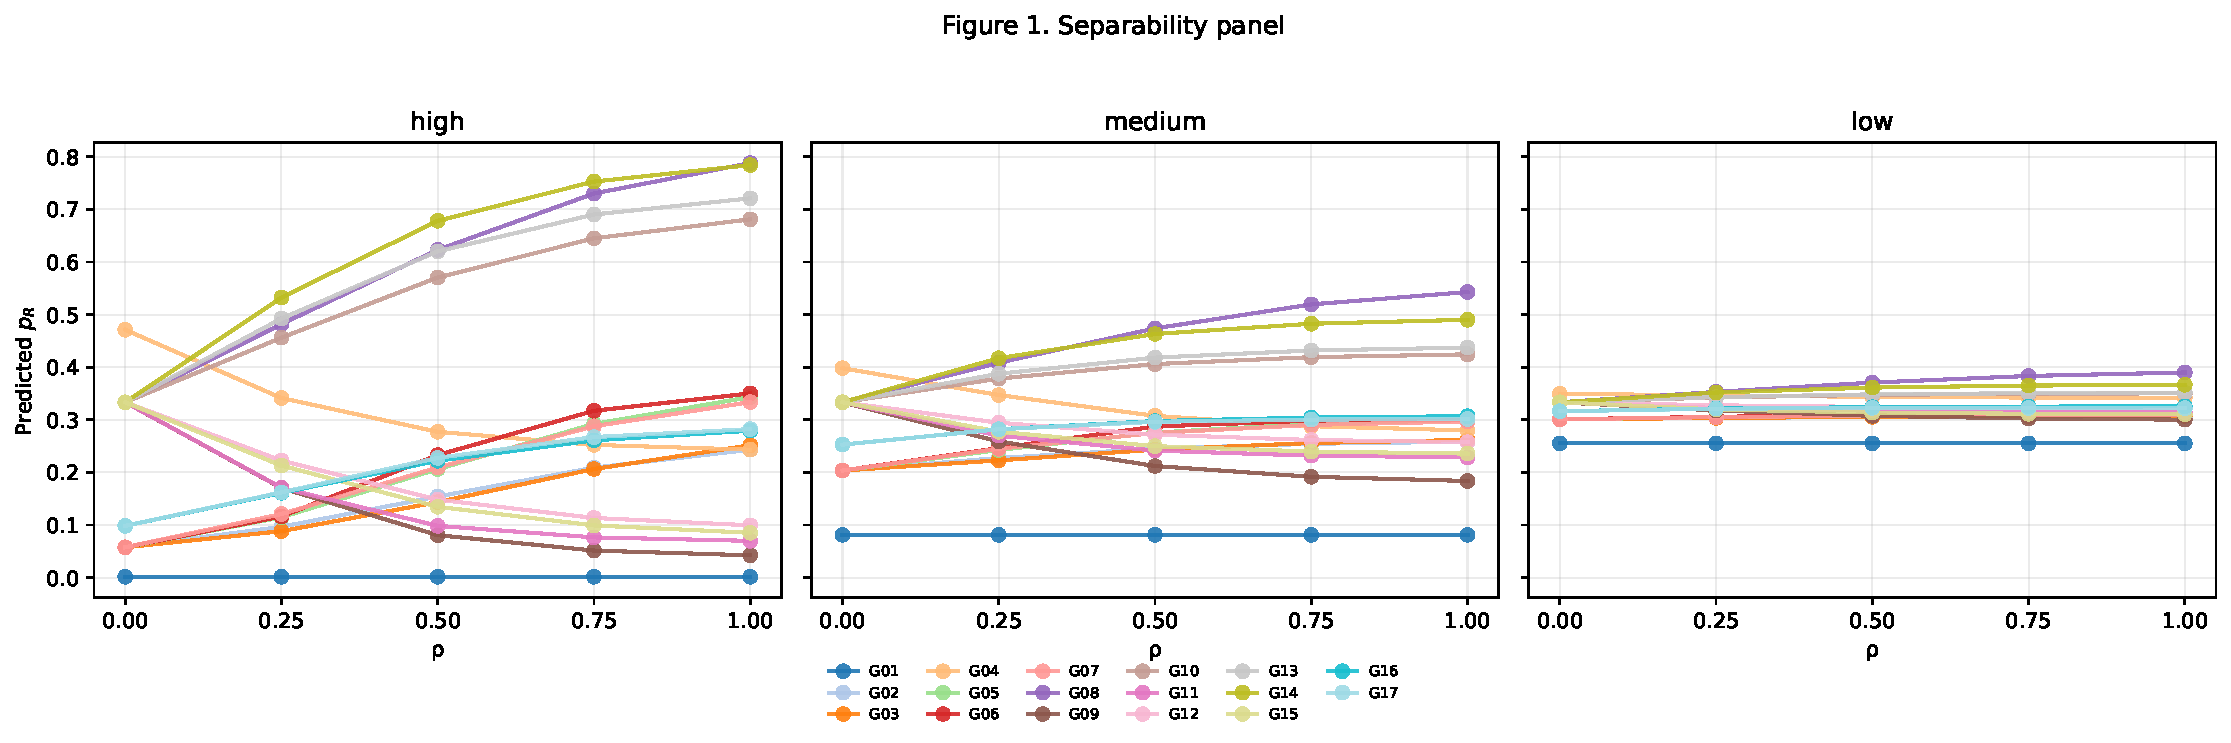
\includegraphics[width=0.98\textwidth]{analysis-2_fig1_separability_panel.pdf}
\caption{Figure 1. 对每个 evidence level，画出 17 张图的 $p_R$--$\rho$ 曲线。除 4-star 退化图外，其余图的 5 个 $\rho$ 水平均可分离。}
\end{figure}

\begin{figure}[ht]
\centering
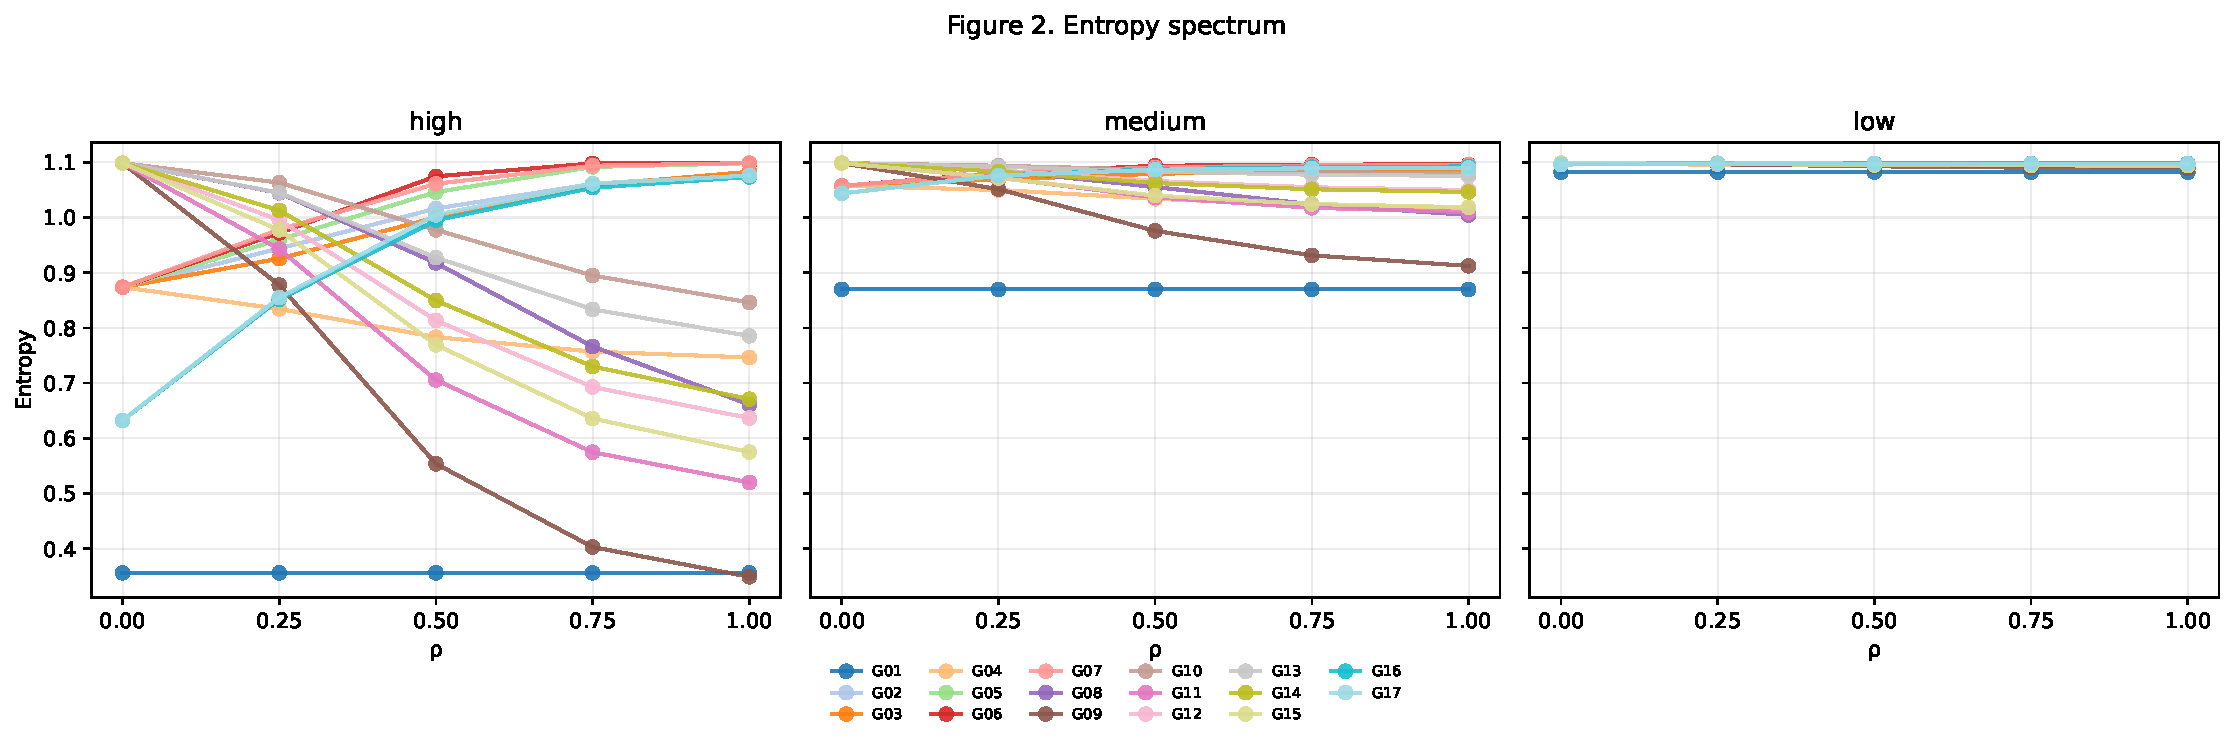
\includegraphics[width=0.98\textwidth]{analysis-2_fig2_entropy_spectrum.pdf}
\caption{Figure 2. 对每个 evidence level，画出 17 张图的响应熵谱。adaptive conflicting 设计下，熵随 $\rho$ 呈稳定的单调变化。}
\end{figure}

\begin{figure}[p]
\centering
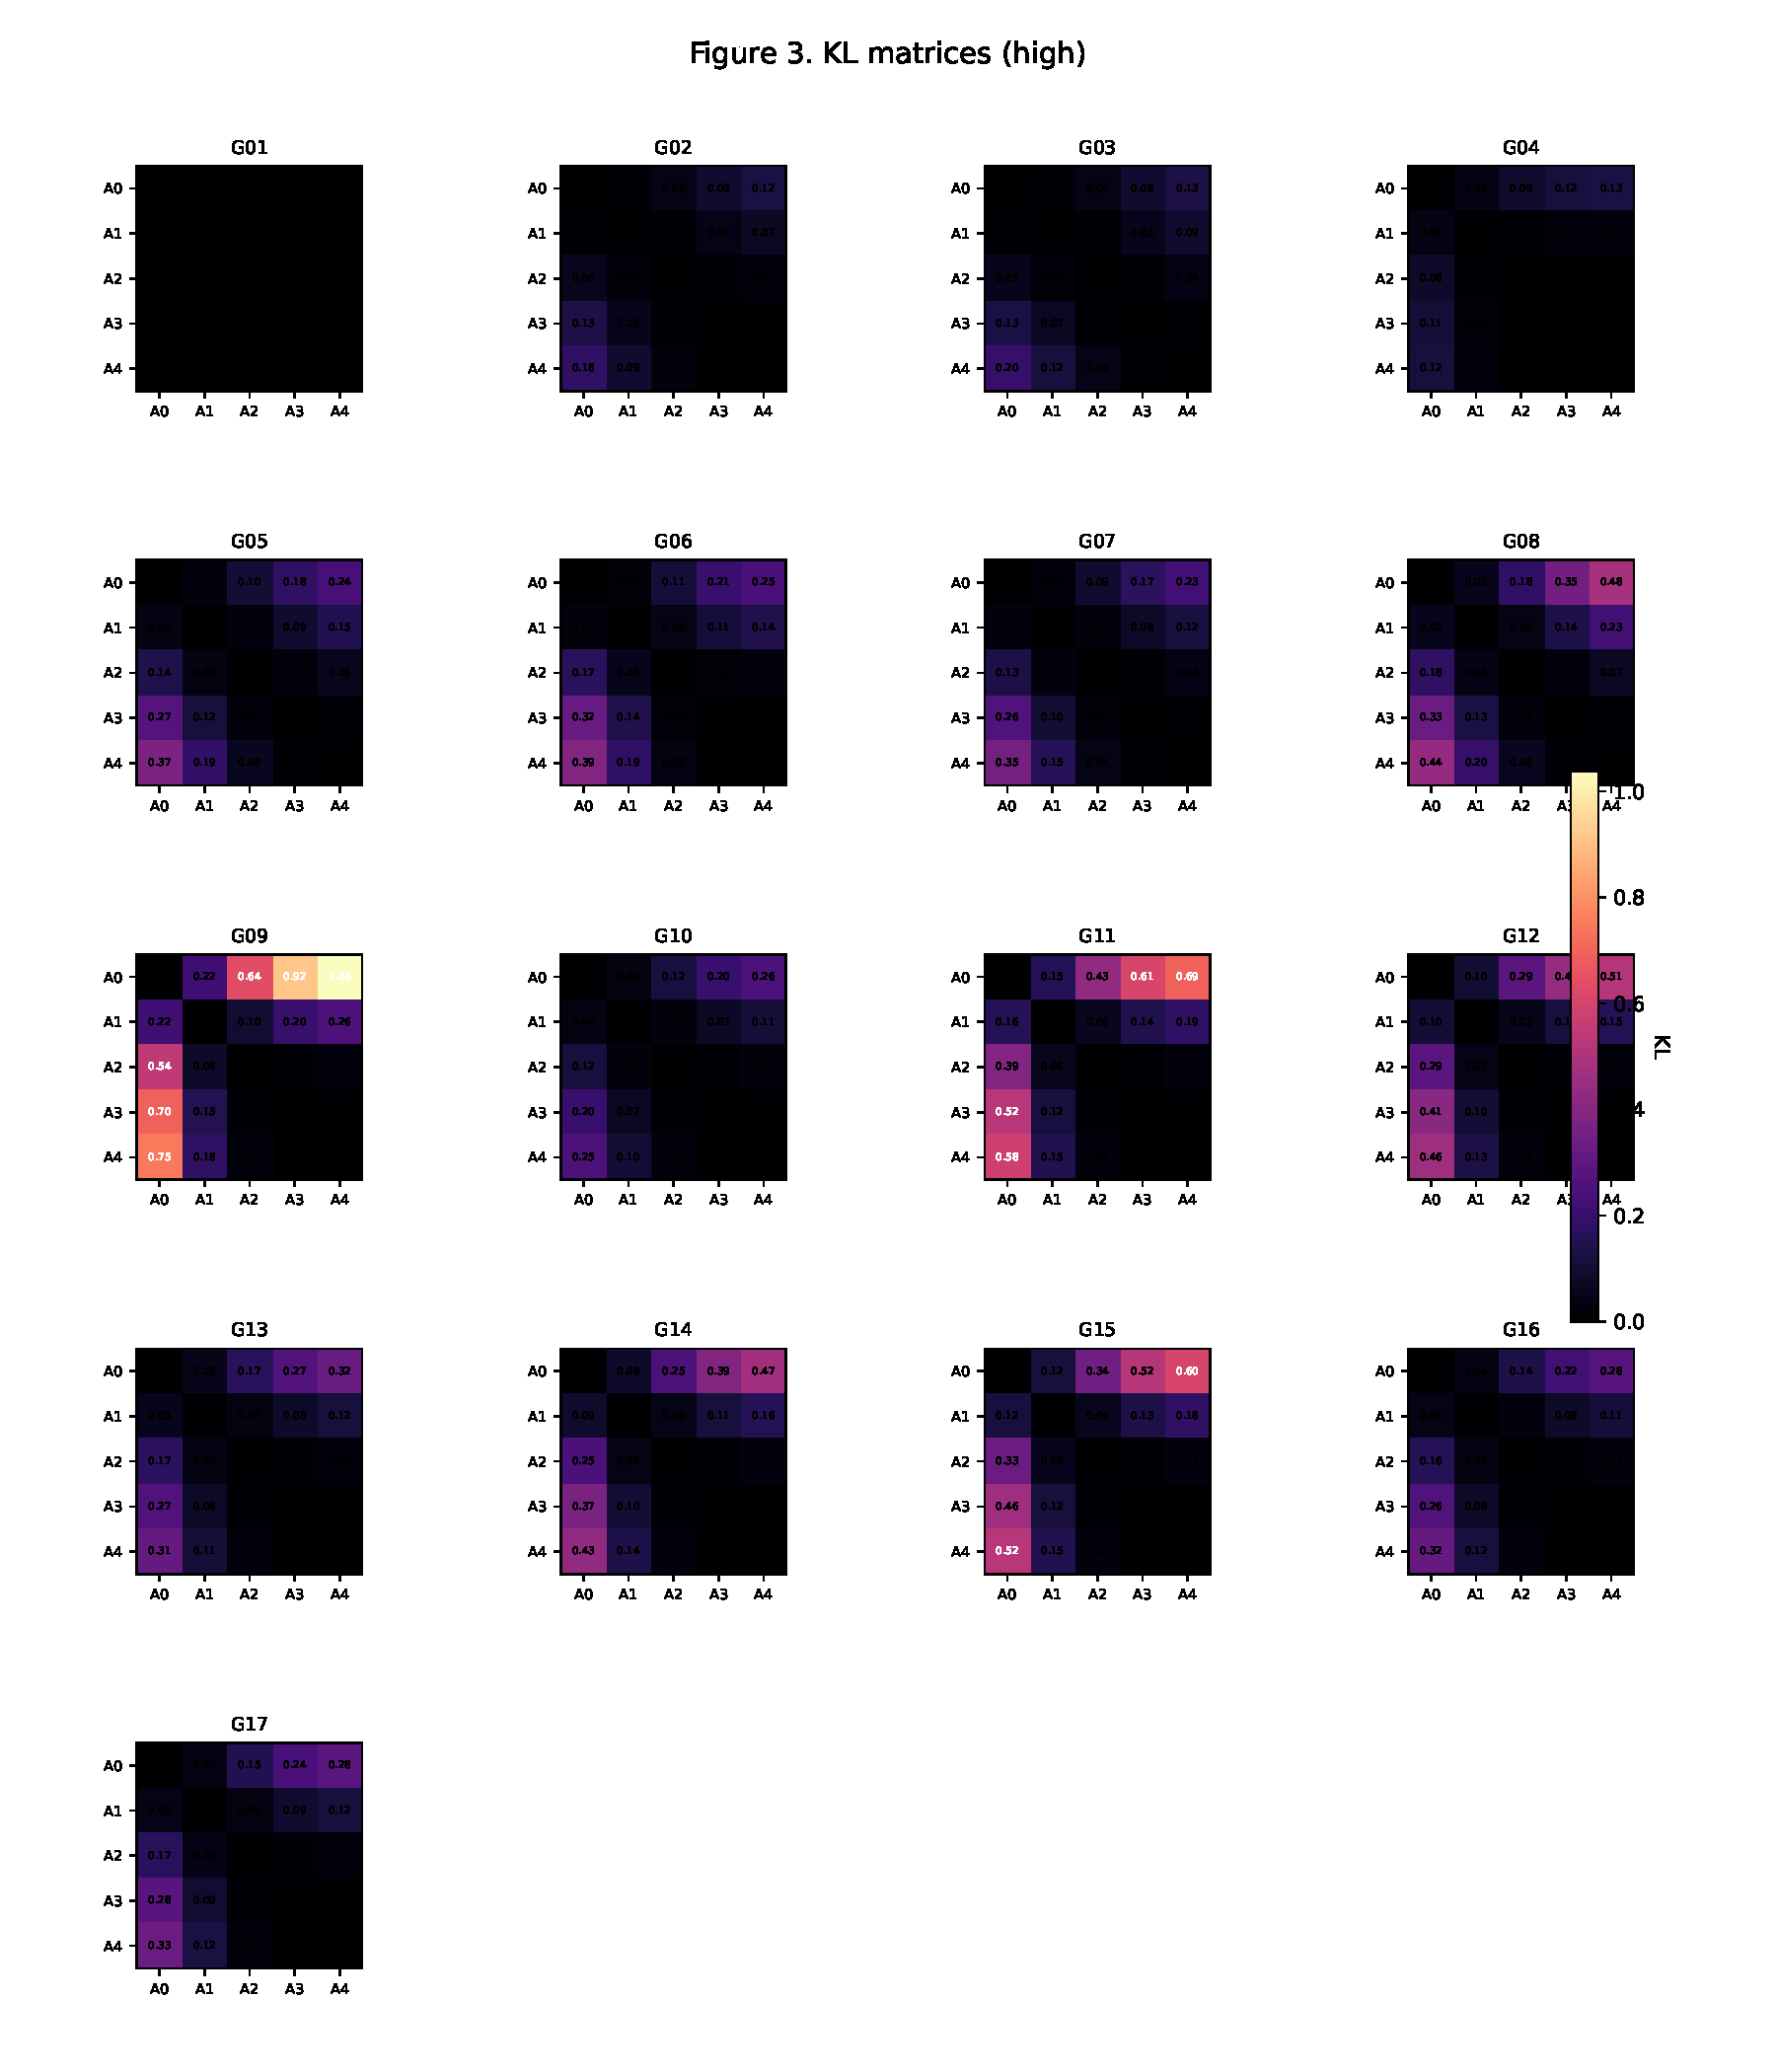
\includegraphics[page=1,width=0.98\textwidth]{analysis-2_fig3_kl_matrices.pdf}
\caption{Figure 3a. high evidence 下每张图的 5$\times$5 directed KL matrix。颜色越深，两个 $\rho$ 代理越容易区分。}
\end{figure}

\begin{figure}[p]
\centering
\includegraphics[page=2,width=0.98\textwidth]{analysis-2_fig3_kl_matrices.pdf}
\caption{Figure 3b. medium evidence 下的 directed KL matrix。}
\end{figure}

\begin{figure}[p]
\centering
\includegraphics[page=3,width=0.98\textwidth]{analysis-2_fig3_kl_matrices.pdf}
\caption{Figure 3c. low evidence 下的 directed KL matrix。整体分离度下降，但多数图仍保持有序谱。}
\end{figure}

\clearpage
\section{Equal-local, distinct-remote 图对}

在最终刺激集中，我们找到了一个非常强的 equal-local 图对：`G08` 与 `G09`。这两张图都让目标节点 $X$ 连接到 3 个 shell-0 evidence 节点，且这 3 个局部节点的颜色偏好完全相同（分别为 $R,B,G$），因此 $A_0$ 在两图上的预测完全一致：
\[
\tilde b_0^{A} = \tilde b_0^{B} = (1/3,1/3,1/3).
\]
但加入 remote structure 后，$A_4$ 在 high evidence 下分裂为
\[
\tilde b_1^{A}=(0.788,0.122,0.090),
\qquad
\tilde b_1^{B}=(0.042,0.915,0.042),
\]
对应的 symmetric KL 达到 3.814，说明远端结构足以在“局部完全相同”的条件下翻转全局预测。

\begin{figure}[ht]
\centering
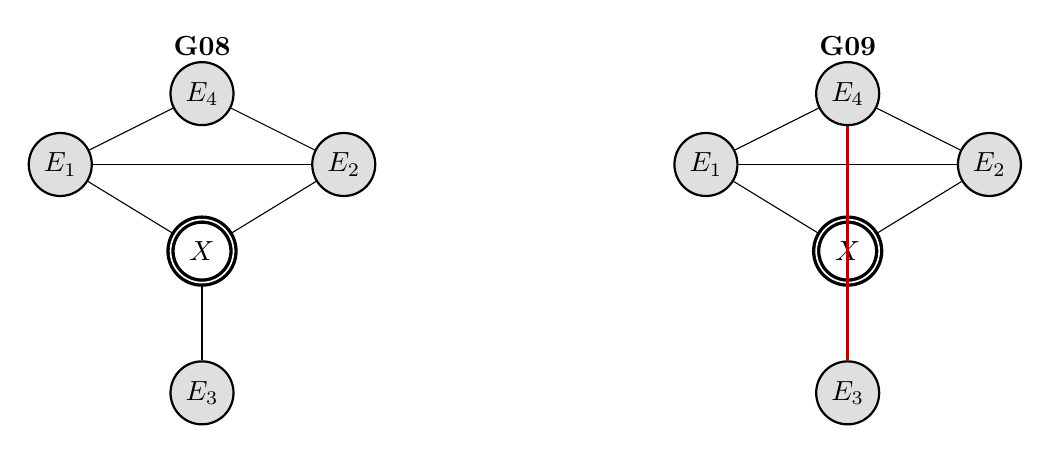
\begin{tikzpicture}[scale=1.0]
    \begin{scope}
        \node at (0,2.6) {\textbf{G08}};
        \node[target]   (xa) at (0,0) {$X$};
        \node[observed] (a1) at (-1.8,1.1) {$E_1$};
        \node[observed] (a2) at (1.8,1.1) {$E_2$};
        \node[observed] (a3) at (0,-1.8) {$E_3$};
        \node[observed] (a4) at (0,2.0) {$E_4$};
        \draw (xa)--(a1);
        \draw (xa)--(a2);
        \draw (xa)--(a3);
        \draw (a1)--(a2);
        \draw (a1)--(a4);
        \draw (a2)--(a4);
    \end{scope}
    \begin{scope}[shift={(8.2,0)}]
        \node at (0,2.6) {\textbf{G09}};
        \node[target]   (xb) at (0,0) {$X$};
        \node[observed] (b1) at (-1.8,1.1) {$E_1$};
        \node[observed] (b2) at (1.8,1.1) {$E_2$};
        \node[observed] (b3) at (0,-1.8) {$E_3$};
        \node[observed] (b4) at (0,2.0) {$E_4$};
        \draw (xb)--(b1);
        \draw (xb)--(b2);
        \draw (xb)--(b3);
        \draw (b1)--(b2);
        \draw (b1)--(b4);
        \draw (b2)--(b4);
        \draw[very thick, red!70!black] (b3)--(b4);
    \end{scope}
\end{tikzpicture}
\caption{用于 Figure 4 的 equal-local 图对。两图的局部邻域完全相同，唯一差异是 G09 多了一条远端边 $E_3$--$E_4$。}
\end{figure}

\begin{figure}[ht]
\centering
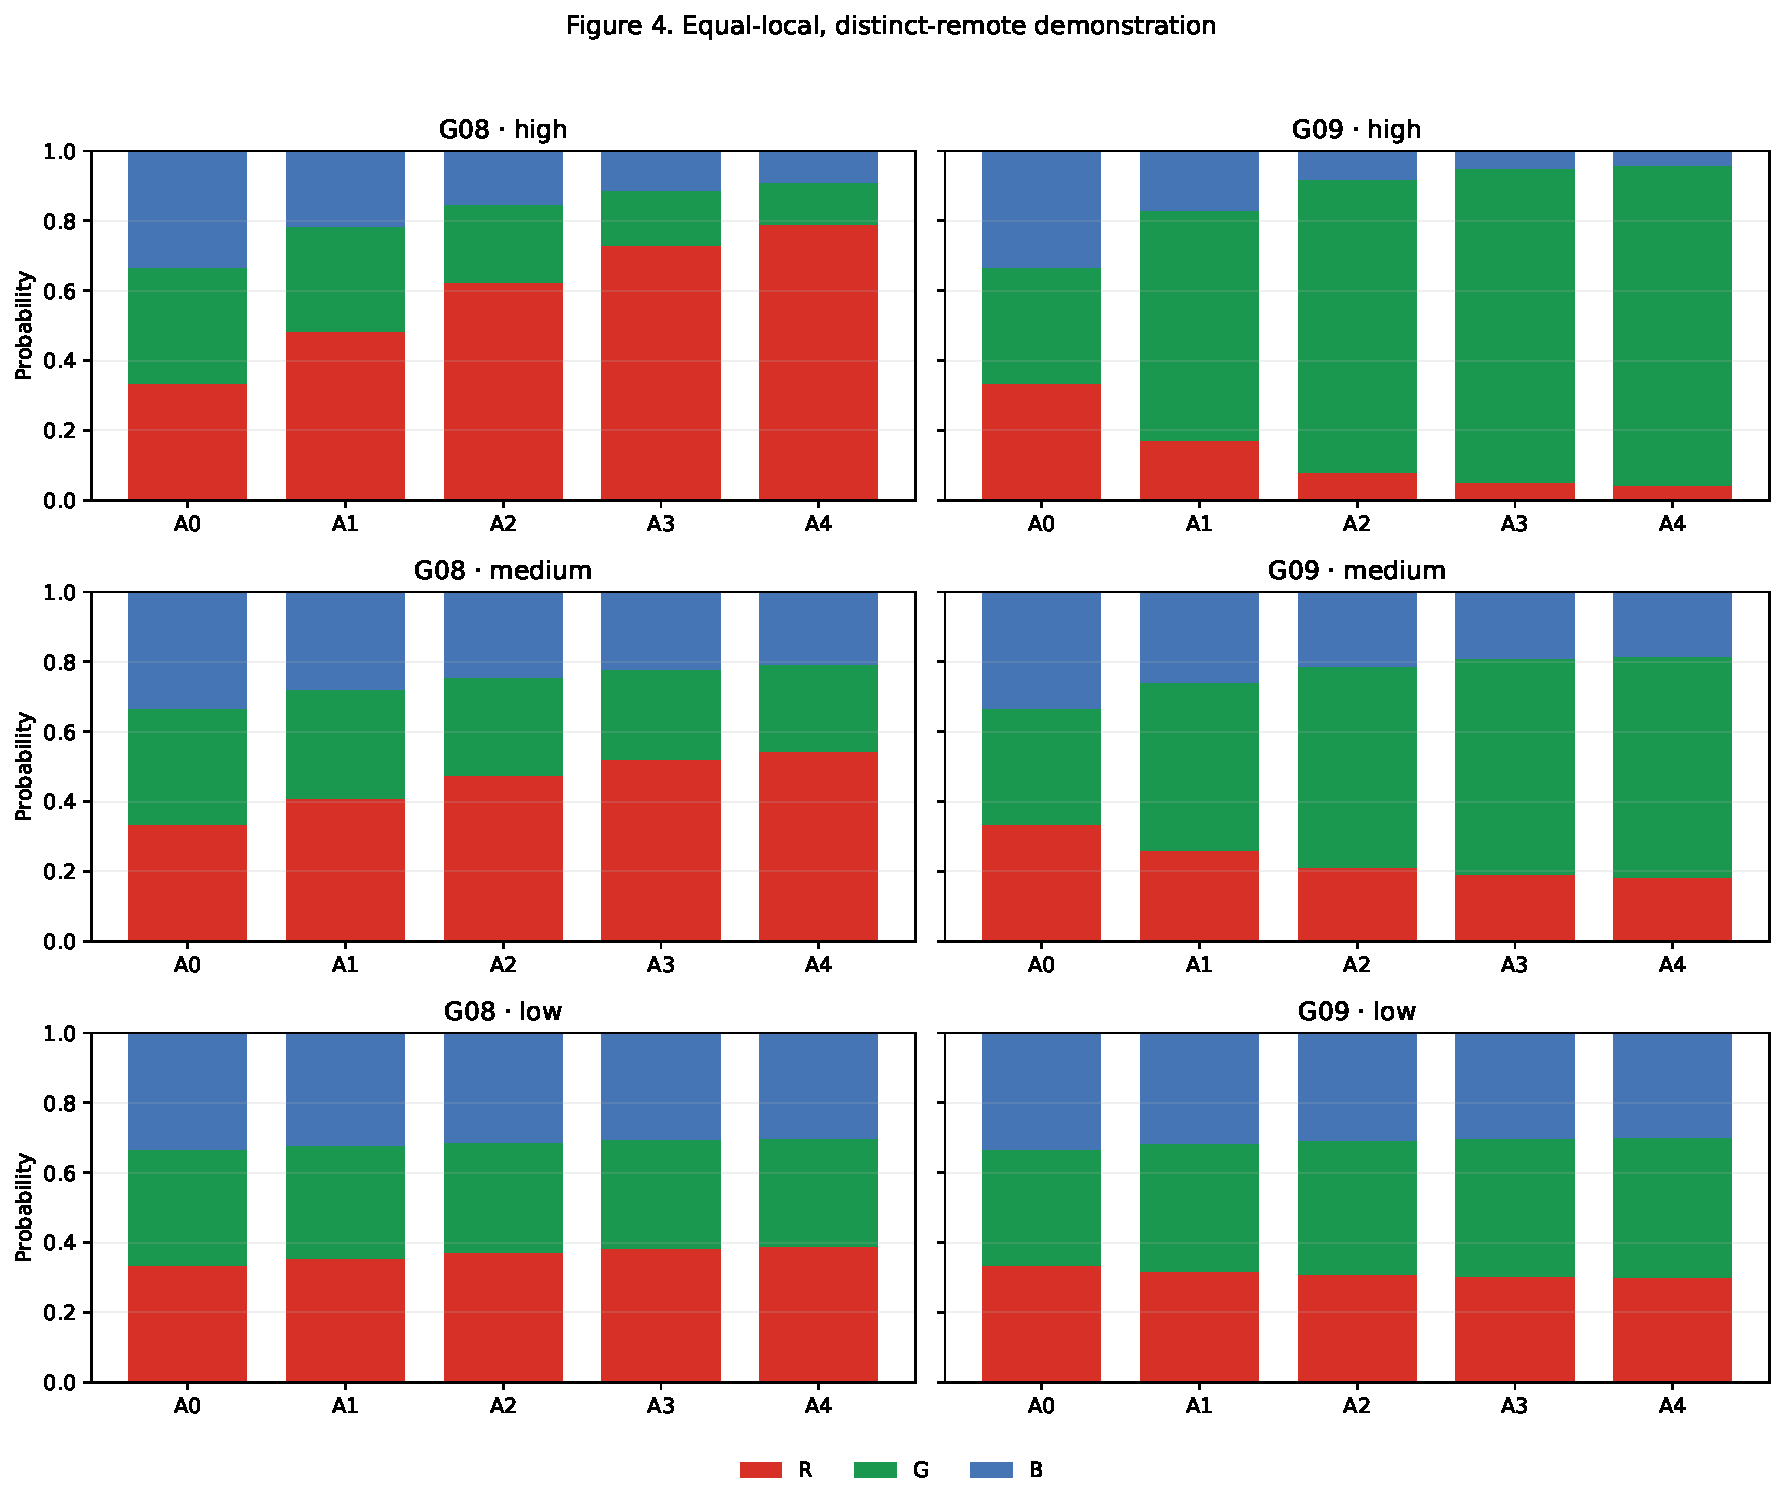
\includegraphics[width=0.92\textwidth]{analysis-2_fig4_equal_local_pair.pdf}
\caption{Figure 4. equal-local 图对的完整预测分布。每个小图都把 5 个代理的 $(p_R,p_G,p_B)$ 画成堆叠条形图。$A_0$ 在两图上完全一致，而高 $\rho$ 代理随远端结构出现强分离。}
\end{figure}

\section{结论}

本分析完整满足 TODO-2 的 3 条成功标准：
\begin{enumerate}
    \item \textbf{Q1 成功。} 17 张 5 节点图中有 16 张在 high evidence 下呈现显著结构分离，说明最小图集已经足以产生可分离预测；无需扩展到 6 节点。
    \item \textbf{Q2 成功。} $\rho=0,0.25,0.5,0.75,1$ 构成的连续谱在完整图集上依然稳定、单调、可解释。
    \item \textbf{equal-local 判别逻辑成功。} 至少存在一对图满足 $\tilde b_0^A=\tilde b_0^B$ 但 $\tilde b_1^A\neq\tilde b_1^B$，而且分离量非常大。
\end{enumerate}

设计层面的实质性结论是：\textbf{conflicting evidence 确实优于 uniform evidence}；进一步地，若把 conflicting 做成按 rooted graph 自适应优化的刺激设计，其总 pairwise separability 比 uniform 提高 3.74 倍，是后续 human experiment 最合适的 5 节点 Phase-1 模拟基线。

\end{document}
